% ****** Start of file apssamp.tex ******
%
%   This file is part of the APS files in the REVTeX 4.2 distribution.
%   Version 4.2a of REVTeX, December 2014
%
%   Copyright (c) 2014 The American Physical Society.
%
%   See the REVTeX 4 README file for restrictions and more information.
%
% TeX'ing this file requires that you have AMS-LaTeX 2.0 installed
% as well as the rest of the prerequisites for REVTeX 4.2
%
% See the REVTeX 4 README file
% It also requires running BibTeX. The commands are as follows:
%
%  1)  latex apssamp.tex
%  2)  bibtex apssamp
%  3)  latex apssamp.tex
%  4)  latex apssamp.tex
%
\documentclass[%
reprint,
%superscriptaddress,
%groupedaddress,
%unsortedaddress,
%runinaddress,
%frontmatterverbose, 
%preprint,
%preprintnumbers,
% nofootinbib,
%nobibnotes,
%bibnotes,
amsmath, amssymb,
aps,
%pra,
%prb,
%rmp,
%prstab,
%prstper,
floatfix,
]{revtex4-2}

\usepackage{graphicx}% Include figure files
\usepackage{dcolumn}% Align table columns on decimal point
\usepackage{bm}% bold math
\usepackage{float}
\usepackage{subcaption}% Subcaption for figures

\usepackage[T1]{fontenc}
\usepackage[utf8]{inputenc}
\usepackage{babel}

%\usepackage{hyperref}% add hypertext capabilities
%\usepackage[mathlines]{lineno}% Enable numbering of text and display math
%\linenumbers\relax % Commence numbering lines

%\usepackage[showframe,%Uncomment any one of the following lines to test 
%%scale=0.7, marginratio={1:1, 2:3}, ignoreall,% default settings
%%text={7in,10in},centering,
%%margin=1.5in,
%%total={6.5in,8.75in}, top=1.2in, left=0.9in, includefoot,
%%height=10in,a5paper,hmargin={3cm,0.8in},
%]{geometry}

\begin{document}

\preprint{APS/123-QED}

\title{Using a Liquid Xenon Positron Target}% Force line breaks with \\
% \thanks{A footnote to the article title}%

\author{Max Varverakis}
\email{mvarvera@calpoly.edu}
\affiliation{California Polytechnic State University, San Luis Obispo, CA 93407, USA}
\author{Spencer Gessner}%
\email{sgess@slac.stanford.edu}
\affiliation{SLAC National Accelerator Laboratory, Menlo Park, California 94025, USA}%

% \collaboration{MUSO Collaboration}%\noaffiliation

% \author{Charlie Author}
%  \homepage{http://www.Second.institution.edu/~Charlie.Author}
% \affiliation{
%  Second institution and/or address\\
%  This line break forced% with \\
% }%
% \affiliation{
%  Third institution, the second for Charlie Author
% }%
% \author{Delta Author}
% \affiliation{%
%  Authors' institution and/or address\\
%  This line break forced with \textbackslash\textbackslash
% }%

% \collaboration{CLEO Collaboration}%\noaffiliation

\date{\today}

\begin{abstract}
ABSTRACT
\begin{description}
\item[Usage]
Secondary publications and information retrieval purposes.
\item[Structure]
You may use the \texttt{description} environment to structure your abstract;
use the optional argument of the \verb+\item+ command to give the category of each item. 
\end{description}
\end{abstract}

%\keywords{Suggested keywords}%Use showkeys class option if keyword display desired
\maketitle

%\tableofcontents

% \section{Outline}
% \begin{itemize}
%     \item Introduction
%     \begin{itemize}
%         \item What is the problem that we are trying to solve?
%         \item What are the issues with "traditional" positron targets?
%         \item What approaches have been tried already?
%         \item How many positrons-per-second are needed for Linear Collider applications?
%         \item Introduction is basically a literature survey/review.
%     \end{itemize}
%     \item Comparing Positron production in Xenon vs W or Ta
%     \begin{itemize}
%         \item This is where the GEANT simulations go.
%         \item How thick/dense does Xenon need to be to match positron production in W or Ta?
%     \end{itemize}
%     \item Cryo-cooled Xenon gas jets
%     \begin{itemize}
%         \item Does this exist?
%         \item Describe work with liquid Xenon and work with cryo-cooled gas jets at SLAC.
%         \item Vacuum challenges?
%     \end{itemize}
%     \item Conclusion
%     \begin{itemize}
%         \item Describe next steps. How would we actually build/implement this?
%     \end{itemize}
    
% \end{itemize}

\section{Introduction}
A common scheme for producing positrons is by colliding high energy electrons into a high-Z target.
The collision between an electron beam and a solid target generates an electromagnetic particle shower,
in which positrons are produced.
Because the collision is such high energy, a great deal of energy is deposited in the target in the form of
thermal energy.  As a result, solid targets tend to degrade over time [].  Since positron yield increases as a
function of radiation length [], a thicker the target implies a greater positron yield, but that also implies
a greater energy will deposited into the target, leading to a quicker degredation of the target.

There are various methods for increasing
the life span of solid targets, such as using a cooling system [] and rotating the target so that the beam doesn't
hit the same spot of the target every pulse [].

Previous experiments have been carried out to explore alternatives to using solid targets, such as using liquid Mercury (Hg),
but the apparent hazards that Hg presents are too dangerous to implement in any efficient manner.
Other approaches include...

For typical Linear Collider applications, around *** $e^+$ per second need to be produced [].

In this paper, we explore the possibility of using a liquid Xenon (Xe) target to produce positrons.

\section{Simulation Results}
\subsection{Comparing Liquid Xe and Ta Targets}
Comparison study between Tantalum (Ta) and liquid Xe because we have a reference study on Ta [].
We used GEANT4 to simulate the collision between 10 GeV $e^-$ and a target.  We compare the results of using a
Ta target and a liquid Xe target.

See Table \ref{tab:G4Params} for parameters used in the simulation.
\begin{table}[h]
    \centering
    \begin{tabular}{cccc}
        \hline \hline
        Material & Z & Density [$\textrm{g} \cdot \textrm{cm}^{-3} $] & Radiation Length [cm] \\
        \hline
        Tantalum (Ta) & 73 & 16.654 & 0.4094 \\
        % \hline
        Liquid Xe (Xe) & 54 & 2.953 & 2.872 \\
        \hline \hline
    \end{tabular}
    \caption{\label{tab:G4Params}Parameters used in GEANT4 simulation when comparing targets.}
\end{table}

\begin{figure}[h]
    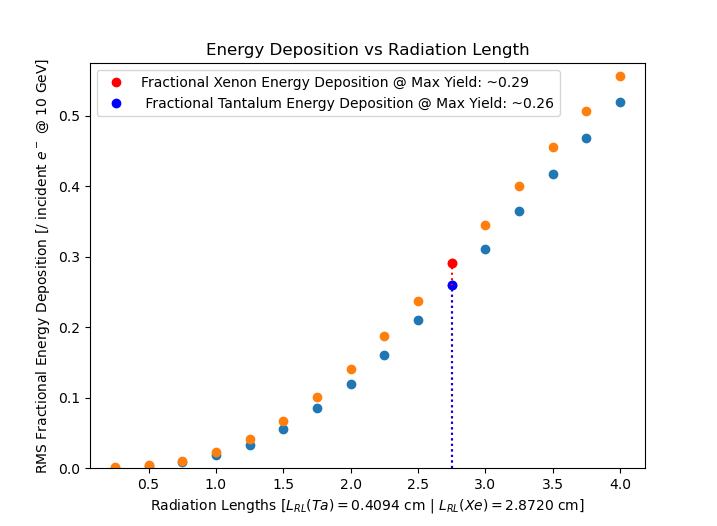
\includegraphics[width = \linewidth]{../images/CompDeps.png}
    \caption{\label{fig:EDep}Energy deposition in Ta and liquid Xe targets per incident electron at 10 GeV.}
\end{figure}

\subsubsection{Calculating Positron Emittance}
To calculate the RMS emittance of the positrons generated in pair production, we utilize the following sets
of equations []
\begin{subequations}
    \begin{eqnarray}
        \left\langle x^2 \right\rangle &= \frac{\sum x^2}{n} - \left( \frac{\sum x}{n} \right)^2, \label{subeq:x2} \\
        \left\langle p_x^2 \right\rangle &= \frac{\sum p_x^2}{n} - \left( \frac{\sum p_x}{n} \right)^2, \label{subeq:p2} \\ 
        \left\langle xp_x \right\rangle &= \frac{\sum xp_x}{n} - \frac{\sum x \sum p_x}{n^2}, \label{subeq:xp}
    \end{eqnarray}
\end{subequations}
which gives us
\begin{equation}
    \varepsilon_{n,rms} = \frac{1}{m_0c}\sqrt[]{\left\langle x^2 \right\rangle \left\langle p_x^2 \right\rangle - \left\langle xp_x \right\rangle}. \label{eq:Emittance}
\end{equation}
Using these equations, we generate a plot of the x- and y-emittance of the positrons against target width for both
Tantalum and liquid Xenon targets.  As seen in Figure \ref{fig:Emittance}, both the x- and y-emittance of the positrons
are lower in the Tantalum target than in the liquid Xenon target.  According to [], the emittance values associated
with liquid Xenon are still comparable for use in linear colliders.
\begin{figure}[h]
    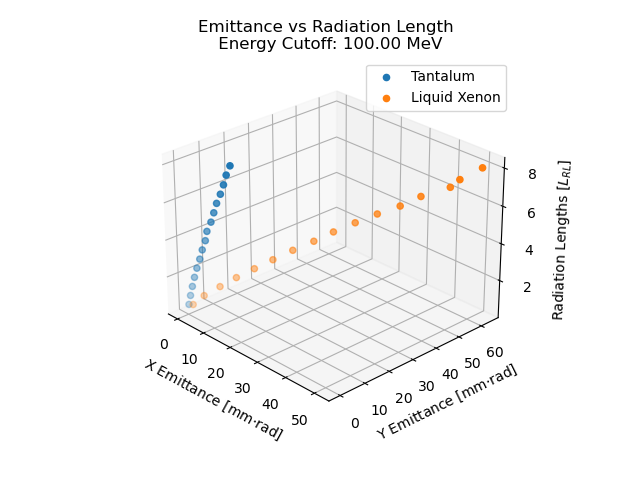
\includegraphics[width = .825\linewidth]{../images/CompEmittance.png}
    \caption{\label{fig:Emittance}Normalized RMS positron emittance in a Tantalum and liquid Xenon target for differing target widths.
    The positron energy cutoff was set to 100 MeV.}
\end{figure}
% \begin{figure}[h]
%     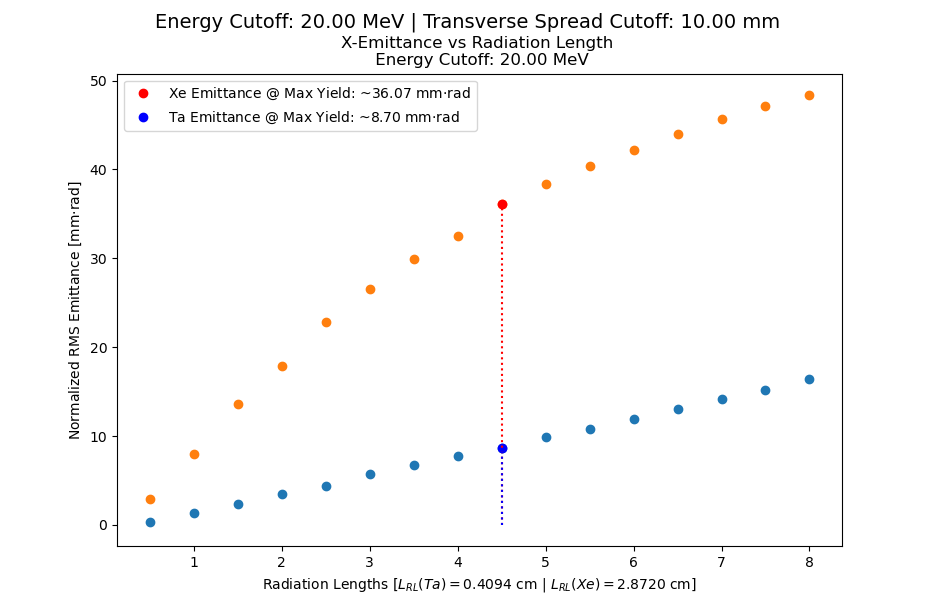
\includegraphics[width = \linewidth]{../images/XCompEmittance.png}
%     \caption{\label{fig:Emittance}RMS positron x-emittance in a Tantalum and liquid Xenon target for differing target widths.
%     The positron energy cutoff was set to 100 MeV.}
% \end{figure}
% \begin{figure}[h]
%     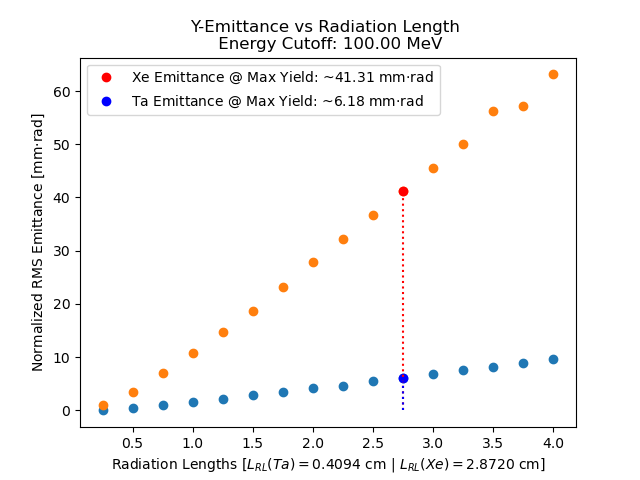
\includegraphics[width = \linewidth]{../images/YCompEmittance.png}
%     \caption{\label{fig:Emittance}RMS positron y-emittance in a Tantalum and liquid Xenon target for differing target widths.
%     The positron energy cutoff was set to 100 MeV.}
% \end{figure}

\begin{figure}[H]
    \begin{subfigure}{.5\textwidth}
        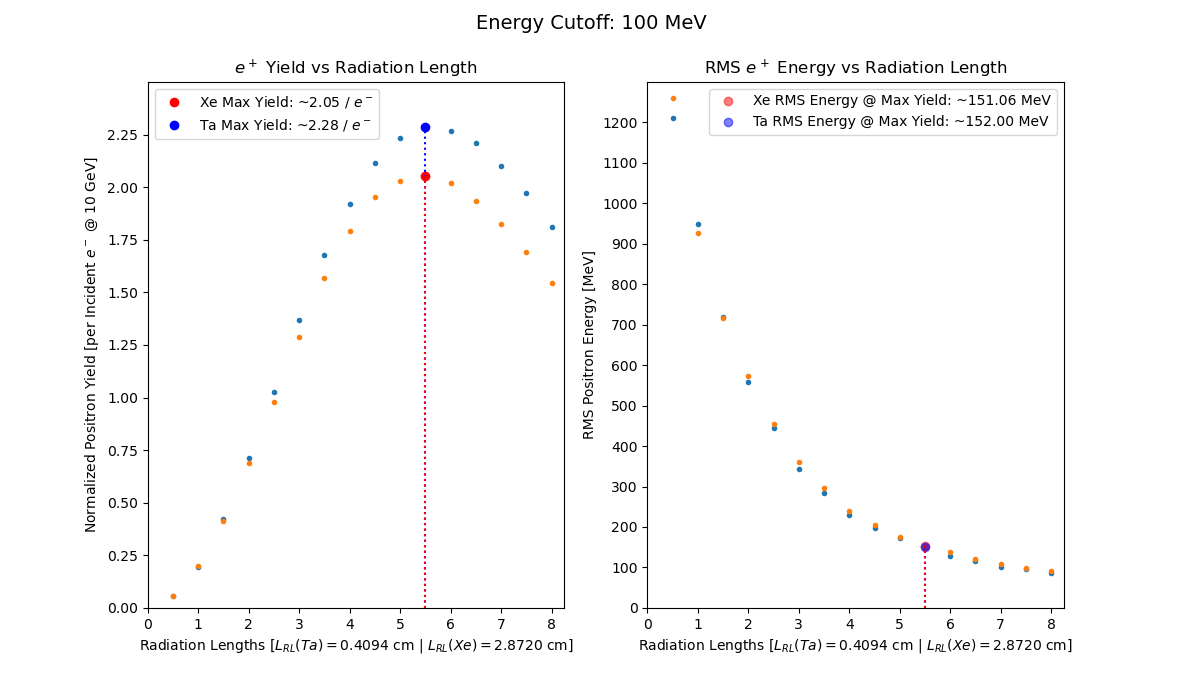
\includegraphics[height = .5\linewidth]{../images/CompYield.png}
        \caption{\label{fig:Yield} Positron yield per incident electron at 10 GeV.}
        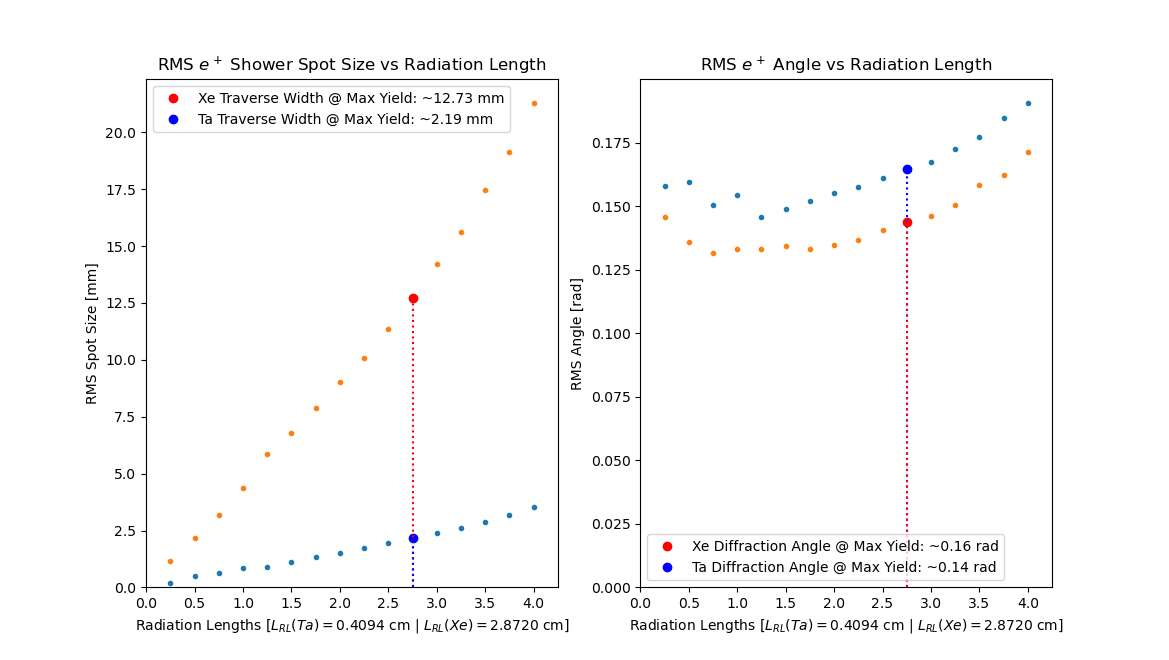
\includegraphics[height = .5\linewidth]{../images/CompATW.png}
        \caption{\label{fig:ATW}Positron shower spot size and diffraction angle at the exit of the target.}
    \end{subfigure}
    \caption{\label{fig:Comps}Positron yield per incident $e^-$ at 10 GeV, 
    shower spot size, and angular divergence of positrons upon exiting the target.}
\end{figure}
From Figure \ref{fig:Yield}, the max positron yield for both Ta and liquid Xe occurs at around 2.75 radiation lengths.
Despite having different radiation lengths, the energy of the positrons exiting the
target at a given width are relatively equal for both target materials.

\begin{figure}[H]
    \begin{subfigure}{.5\textwidth}
        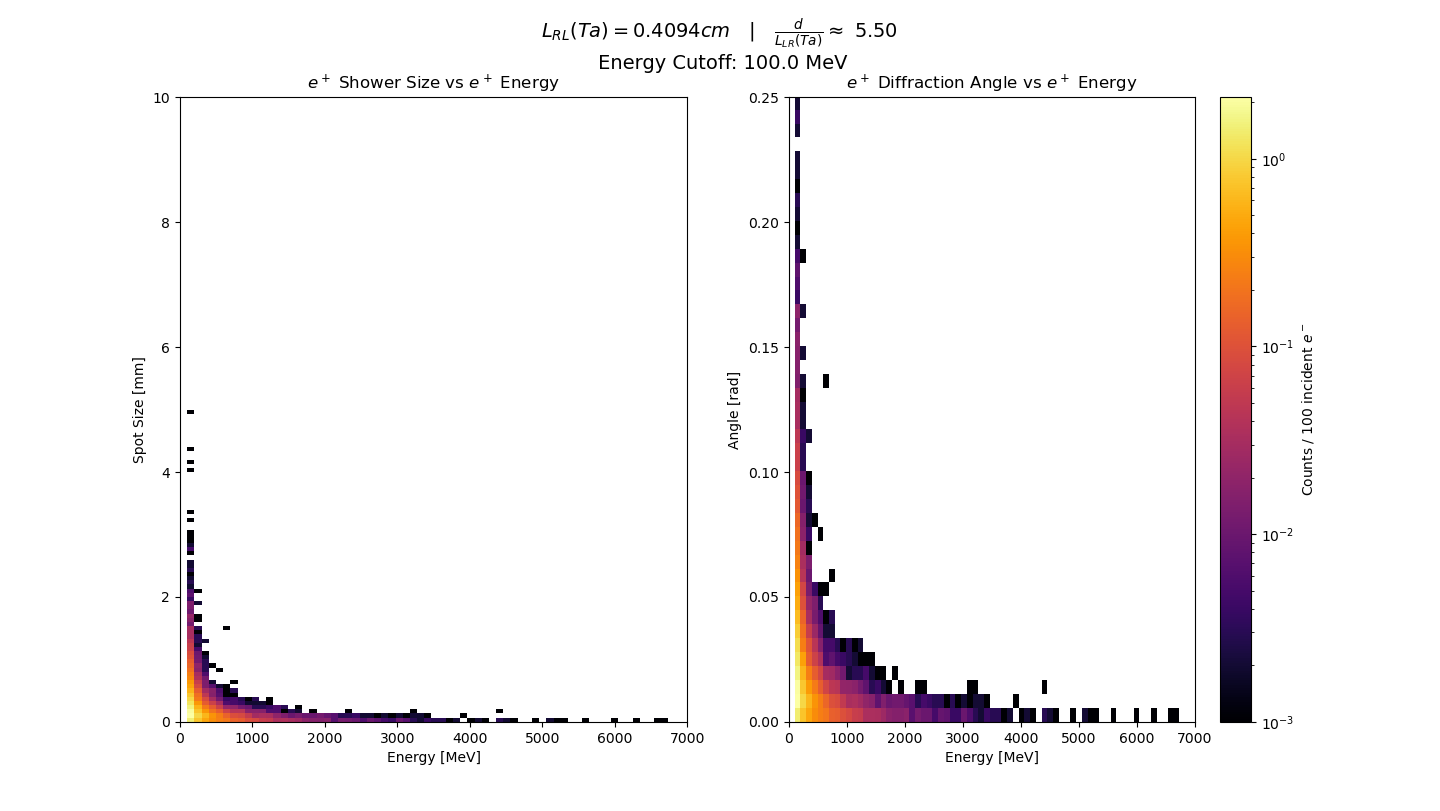
\includegraphics[height = .65\linewidth]{../images/TaHists.png}
        \caption{\label{fig:TaHists}Tantalum target.}
        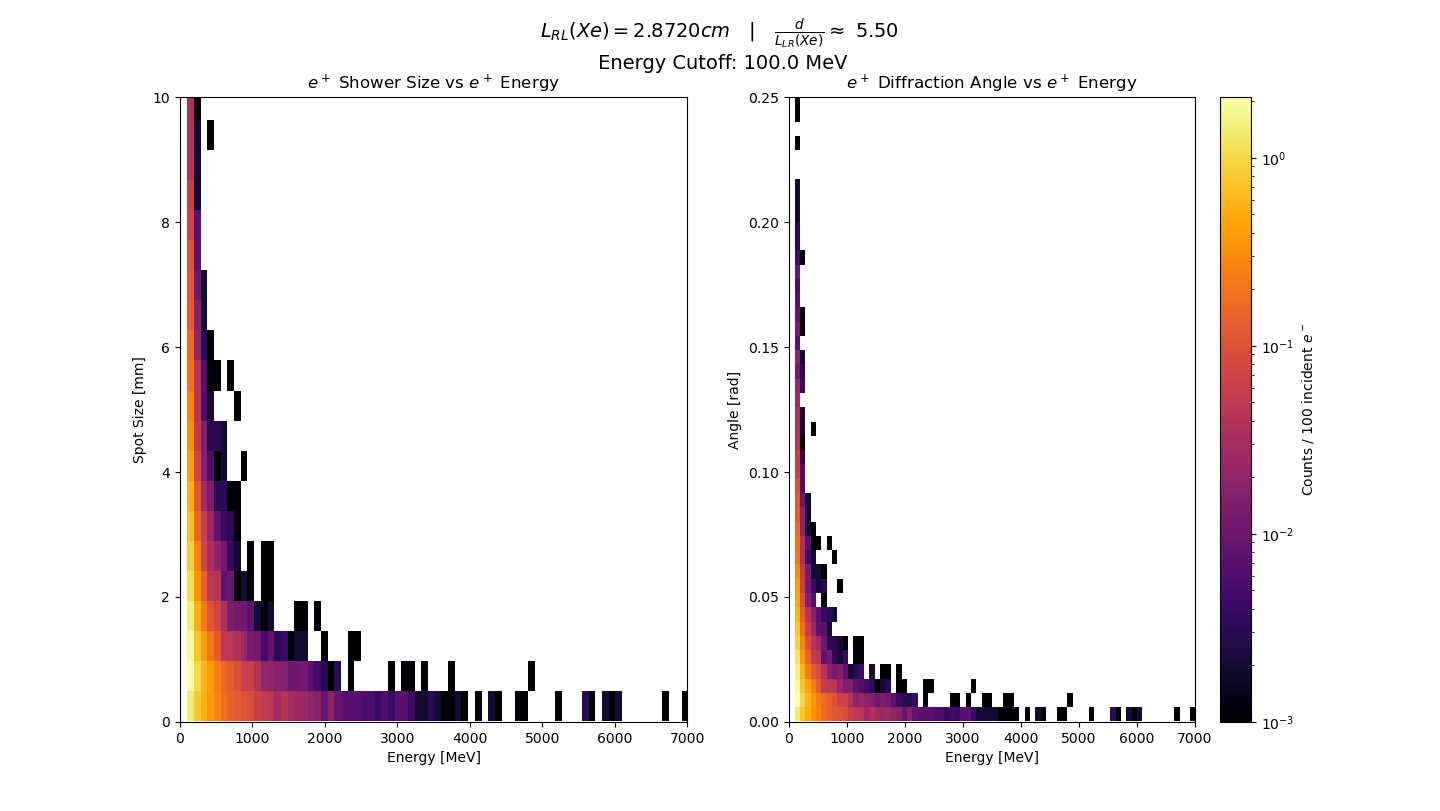
\includegraphics[height = .65\linewidth]{../images/XeHists.png}
        \caption{\label{fig:XeHists}Liquid Xenon target.}
    \end{subfigure}
    \caption{\label{fig:Hists}Traverse width and angular diffraction of positrons as a function
    of their energy upon production.  Data is shown for widths of 2.75 radiation lengths (max e$^+$ yield).}
\end{figure}

Notice that in Figure \ref{fig:Hists}, the angular divergence of positrons is roughly the same for both targets,
yet the traverse widths are more broadly distributed for the liquid Xenon target.  This can be explained by the 
fact that the radiation length of liquid Xenon is roughly seven times that of Tantalum.
\subsection{Setting a Cutoff Traverse Width}
Although the max yield for liquid Xenon is on par with that of the Tantalum target
according to Figures \ref{fig:ATW} and \ref{fig:Hists}, the physical spread of positrons produced
from the liquid Xenon target is much larger than that of the Tantalum target.  As a result, only a
fraction of the positrons that exit the target will have the right characteristics to make it down the rest of
the accelerator.  In order to accurately assess the plausibility of using a liquid Xenon positron target,
we set cutoffs for the traverse width of positrons created during the collision.

\begin{figure}[H]
    \begin{subfigure}{.45\textwidth}
        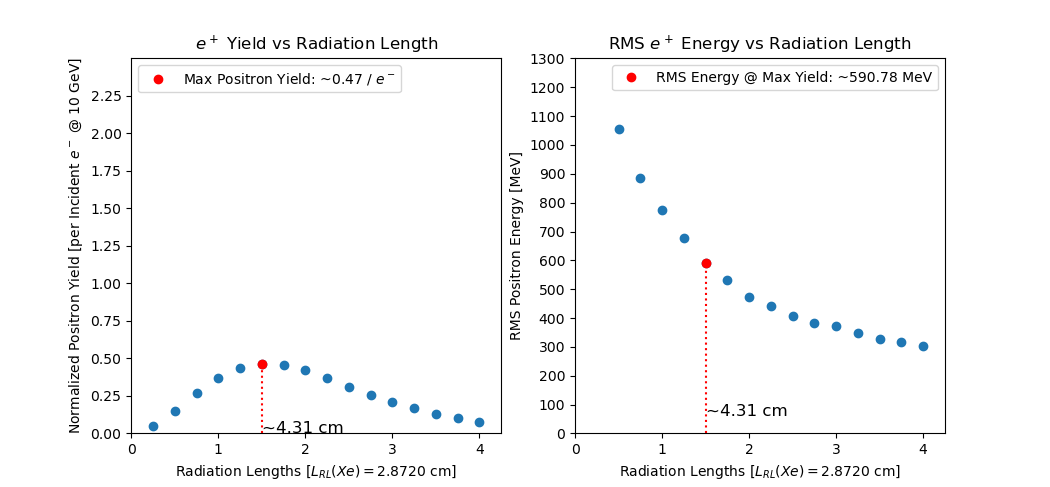
\includegraphics[height = .43\linewidth]{../images/XeYield1mmCutoff.png}
        \caption{\label{fig:XeY1}1 mm cutoff}
        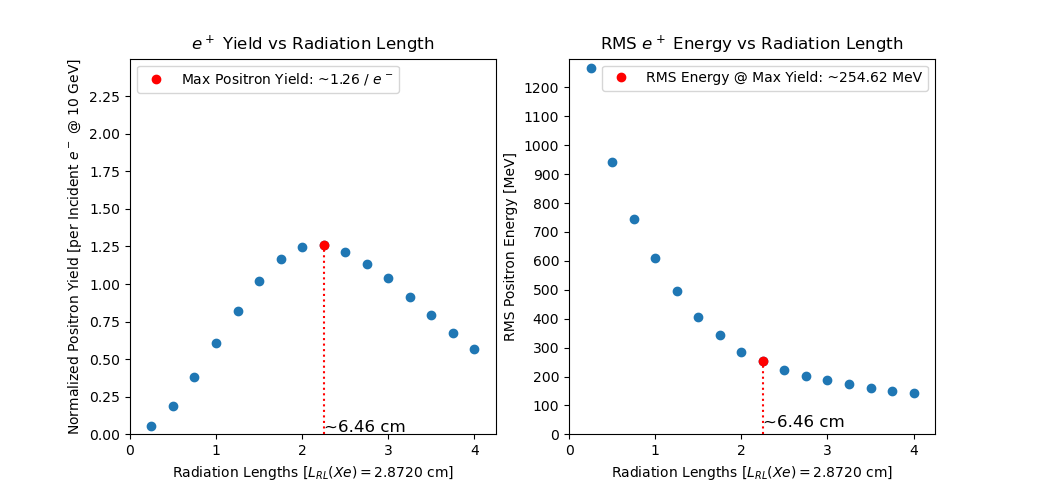
\includegraphics[height = .43\linewidth]{../images/XeYield5mmCutoff.png}
        \caption{\label{fig:XeY5}5 mm cutoff}
    \end{subfigure}
    \caption{\label{fig:YieldCut}Positron yield and energy using 
    a liquid Xenon target with a 1 mm and 5 mm traverse width cutoff.}
\end{figure}

\begin{figure}[H]
    \begin{subfigure}{.5\textwidth}
        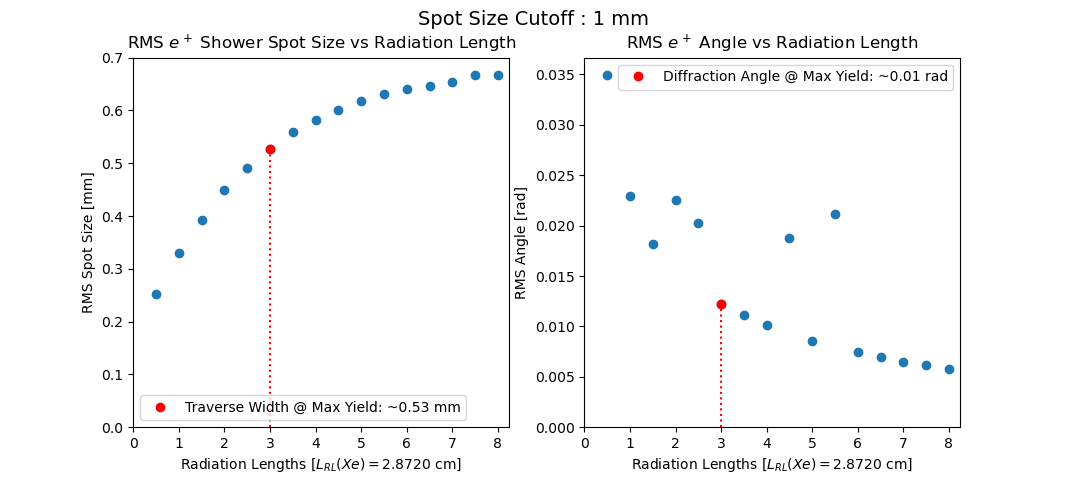
\includegraphics[height = .445\linewidth]{../images/XeATW1mmCutoff.png}
        \caption{\label{fig:XeATW1}1 mm cutoff}
        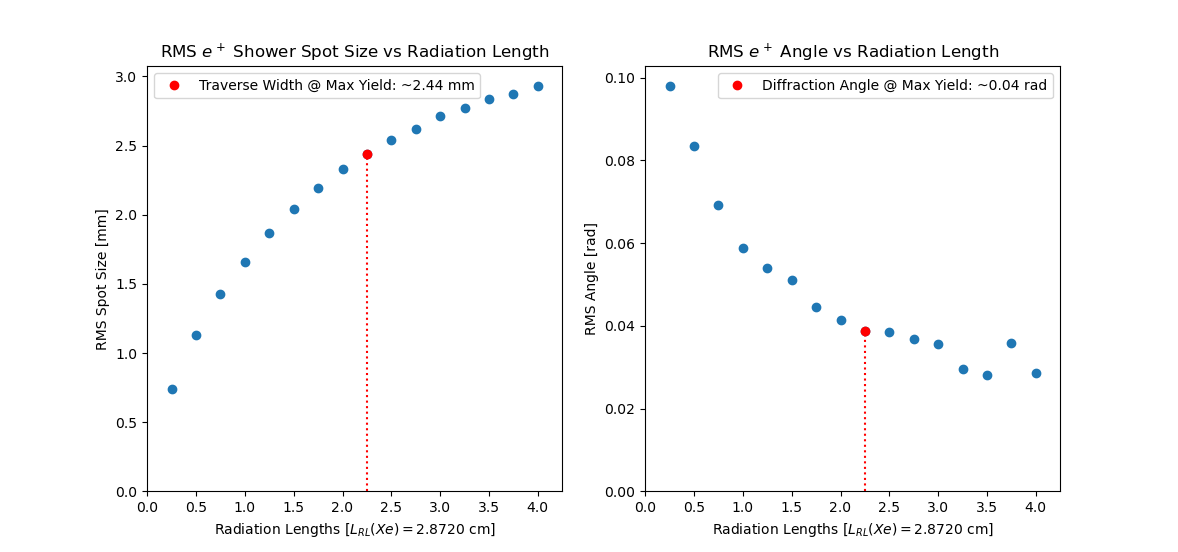
\includegraphics[height = .5\linewidth]{../images/XeATW5mmCutoff.png}
        \caption{\label{fig:XeATW5}5 mm cutoff}
    \end{subfigure}
    \caption{\label{fig:ATWCut}Positron spot size and angular diffraction using 
    a liquid Xenon target with a 1 mm and 5 mm traverse width cutoff.}
\end{figure}
It is reassuring to see that even after removing the positrons from the dataset 
with large transverse distances from the beam path, there are still a comparable number
of positrons that we predict will be able to make it to the next stage of the accelerator [].

\section{Cryo-cooled Liquid Xenon Chamber}
Figure \ref{fig:schem}, a basic schematic of how the liquid Xenon chamber will interact with the beam.
\begin{figure}[H]
    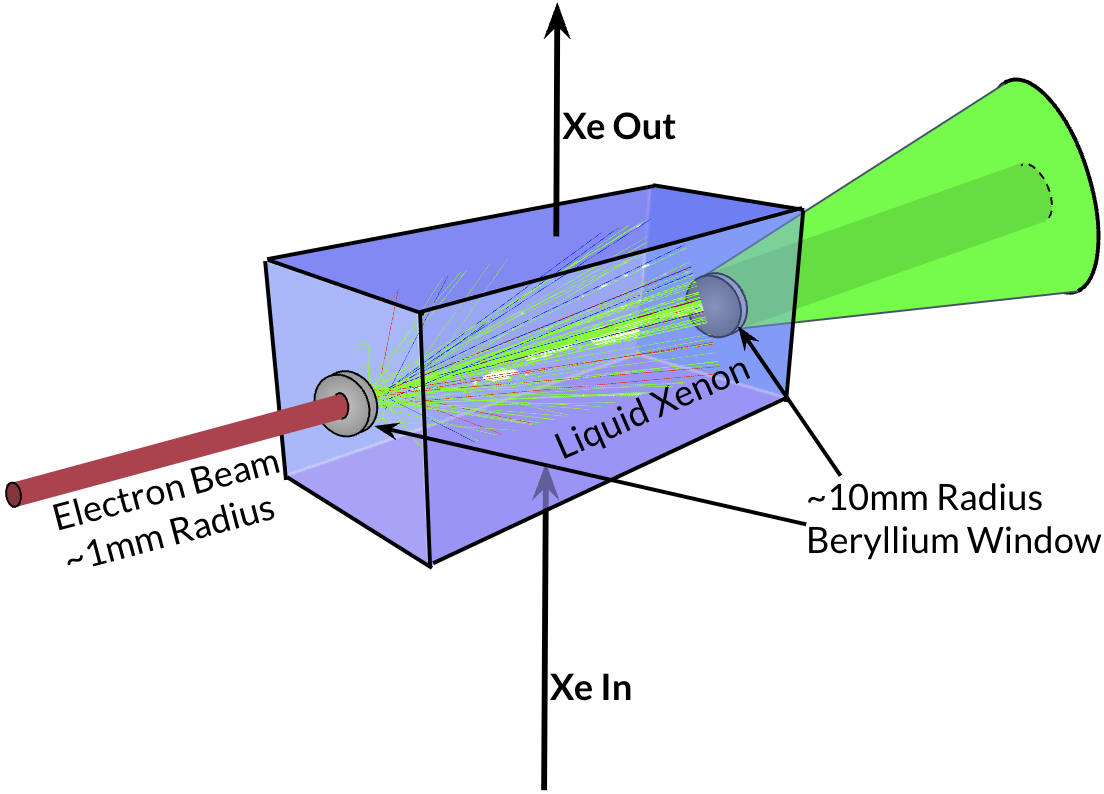
\includegraphics[width = .5\textwidth]{../images/Schematic4.png}
    \caption{\label{fig:schem}Schematic of liquid Xenon setup.}
\end{figure}

\subsection{Calculating the Liquid Xenon Flow Rate}
To calculate the flow rate of the liquid Xenon, we first calculate preliminary
values using the information given in the table below.

\begin{table}[H]
    \centering
    \begin{tabular}{lccc}
        \hline \hline
        \textbf{Liquid Xenon} & \textbf{Symbol} & \textbf{Value} & \textbf{Units} \\
        % Quantity & Symbol & Value & Units \\
        \hline
        % $\textrm{g}\cdot\textrm{mol}^{-1}$
        Molar Mass & M & 131.293 & u \\
        Density & $\rho$ & 2.953 & $\textrm{g} \cdot \textrm{cm}^{-3}$ \\
        Heat of Vaporization & $\Delta \textrm{H}$ & 12.636 & kJ$\cdot$mol$^{-1}$ \\
        Heat of Vap./Volume & $\Delta \textrm{H}_{\textrm{vol}}$ & 284.205 & J$\cdot \textrm{cm}^{-3}$ \\
        Radiation Length & $\textrm{L}_{\textrm{RL}}$ & 2.872 & cm \\
        Width & $\frac{\textrm{d}}{\textrm{L}_{\textrm{RL}}}$ & 5.5 & $\textrm{L}_{\textrm{RL}}$ \\
        % Volume & V & & cm$^3$ \\
        \hline \hline
    \end{tabular}
    \caption{\label{tab:XeInfo}Important parameters associated with liquid Xenon target chamber.}
\end{table}

\begin{table*}
    \centering
    \begin{tabular}{lcccc}
        \hline \hline
        \textbf{Beam Parameters} & \textbf{Symbol} & \textbf{FACET-II} & \textbf{ILC} & \textbf{Units} \\
        \hline
        Energy & $E$ & 10.0 & 6.0 & GeV \\
        Repetition Rate & $f$ & 10 & 300 & Hz \\
        Charge & $q$ & 2 & 3.204 & nC \\
        Number of $e^-$ & n & 1.248 & 2.0 & $10^{10}$ \\
        \hline \hline
        \textbf{Resultant Quantities} \\
        \hline
        Energy Deposition/e$^-$ & E$_{\textrm{dep}}$ & .66581 & & GeV \\
        Energy Deposit/Pulse & $\epsilon$ & 1.332 & 735.9 & J \\
        Energy Deposit Density & $\epsilon_\rho$ & $1.63\times 10^{-3}$ & 3.10 & J$\cdot\textrm{g}^{-1}$ \\
        Power Deposit & $P_\textrm{dep}$ & $3.86$ & $7.359\times 10^8$ & W \\
        Flow Rate due to Vaporization & Q & $4.685 \times 10^{-2}$ & 776.8 & cm$^3\cdot \textrm{s}^{-1}$ \\
        Main Shower Path Flow Rate & $Q_\textrm{vol}$ & 0.6318 & 18.96 & L$\cdot \textrm{s}^{-1}$ \\
        \hline \hline
    \end{tabular}
    \caption{\label{tab:BeamInfo}Linear collider electron beam parameters and associated target quantities [].}
\end{table*}

We first convert the heat of vaporization to units of Joules per unit volume (J$\cdot \textrm{cm}^{-3}$),
which is given by Eq.~(\ref{subeq:HoV}).
We then calculate the number of electrons per beam bunch (SLAC), by comparing the 
total charge of the beam bunch to the charge of an electron
($e \approx 1.602 \times 10^{-10}$ nC), as follows from Eq.~(\ref{subeq:n}).
From this, we calculate the total energy deposited in the liquid Xenon target, 
as seen in Eq.~(\ref{subeq:Etot}).
\begin{subequations}
    \begin{eqnarray}
        \Delta \textrm{H}_\textrm{vol} &=& \frac{\Delta \textrm{H}\cdot \rho}{\textrm{M}}, \label{subeq:HoV} \\
        n &=& \frac{q}{e}, \label{subeq:n} \\
        \epsilon &=& n \cdot E_{\textrm{dep}} \label{subeq:Etot}.
    \end{eqnarray}
\end{subequations}
    
Now we have everything we need in order to calculate the flow rate of liquid Xenon
required to replace the vaporized Xenon due to the energy deposited by the beam,
\begin{equation}
    Q = \frac{\epsilon \cdot f}{\Delta \textrm{H}_{\textrm{vol}}}.
\label{eq:Q}
\end{equation}

In case one wants to calculate the flow rate required to move the entire volume encompassing the main
part of the EM shower, one can approximate the volume with a rectangular prism with target width and other
side lengths equal to the diameter of the Beryllium windows (see next section).  At max positron yield,
this gives $\textrm{V} = (2 \textrm{ cm})^2 \cdot 5.5\textrm{L}_{\textrm{RL}} \approx 63.18 \textrm{ cm}^3$.
As a result, the required flow rate to move volume V in the amount of time between beam pulses is
shown in Table \ref{tab:BeamInfo} as $Q_\textrm{vol}$.

\subsection{Using Beryllium Windows to the Target Chamber}
We explore using Beryllium windows for the beam to enter the target chamber.
Below is some useful information about Beryllium.

\begin{table}[h]
    \centering
    \begin{tabular}{lccc}
        \hline \hline
        \textbf{Beryllium} & \textbf{Symbol} & \textbf{Value} & \textbf{Units} \\
        \hline
        Atomic Number & Z & 4 & \\
        Density & $\rho$ & 1.844 & g$\cdot$cm$^{-3}$ \\
        Rupture Modulus & $F_a$ & 400 & MPa \\
        % Yield Strength & $\sigma_\textrm{y}$ & 240 & MPa \\
        % Tensile Strength & $\sigma_\textrm{t}$ & 370 & MPa \\
        % Shear Strength & $\sigma$ & 1234 & MPa \\
        % Thermal Conductivity & $\kappa$ & 216 & W$\cdot$m$^{-1}$$\cdot$K$^{-1}$ \\
        \hline \hline
        \textbf{Quantities} \\
        \hline
        Height 
        \footnote{Difference in height between the Beryllium window and the top of the liquid Xenon chamber.} 
        & $h$ & 1.0 & m \\
        Radius & $r$ & 10.00 & mm \\
        Contact Area & $A$ & $100\pi$ & mm$^2$ \\
        % Cross Sectional Area & $A_c$ & $2\pi r t$ & mm$^2$ \\
        Pressure & $P$ & 28.968 & kPa \\
        Force & $F$ & 9.100 & N \\
        Safety Factor & $S_F$ & 4 \\
        Empirical Constant & $K$ & 0.75 \\
        Thickness & $T$ & 147.395 & $\mu$m \\
        \hline \hline
    \end{tabular}
    \caption{\label{tab:BeInfo}Useful quantities and properties of solid Beryllium.
    The quantities are specific to a 10mm radius Beryllium disk.}
\end{table}

Utilizing Bernoulli's Equation for conservative force fields [], we can calculate the total
pressure on a Beryllium window, which
is of the form
\begin{equation}
    P = \frac{1}{2} \rho v^2 + \rho g h + p,
\label{eq:Bern}
\end{equation}
where $v$ is the fluid flow rate, $g$ is acceleration due to gravity, $h$ is the height of the Xenon chamber
relative to the height of the window,
and $p$ is the additional pressure from, say, the atmosphere.
However, as seen in Table \ref{tab:BeamInfo}, the flow rate for the liquid Xenon is quite small.  Additionally,
the liquid Xenon chamber is in vacuum, and we are comparing differences in total pressures,
so we can ignore $p$ as well.  Therefore,
we can ignore the second order term and the point-pressure term to further simplify our approximation to
\begin{equation}
    P = \rho g h.
    \label{eq:BernSimp}
\end{equation}

From Eq.~(\ref{eq:BernSimp}), we can calculate the force on a Beryllium window with contact area $A$ by 
multiplying the area by the pressure: $F = P\cdot A$.

In order to determine the required thickness of the Beryllium window, we utilize the following [].
First we calculate a constant related to the safety factor of our thickness, which takes into account
the method with which the Beryllium window is inserted into the target chamber.
An empirical constant $K = 0.75$ is chosen if the window is clamped into the target chamber, and
$K = 1.125$ if the window is unclamped in the target chamber.  For a given safety factor ($S_F$),
we have a thickness of
\begin{equation}
    T = r\cdot\sqrt{\frac{S_F\cdot K\cdot P}{F_a}}.
\end{equation}

\begin{figure}[H]
    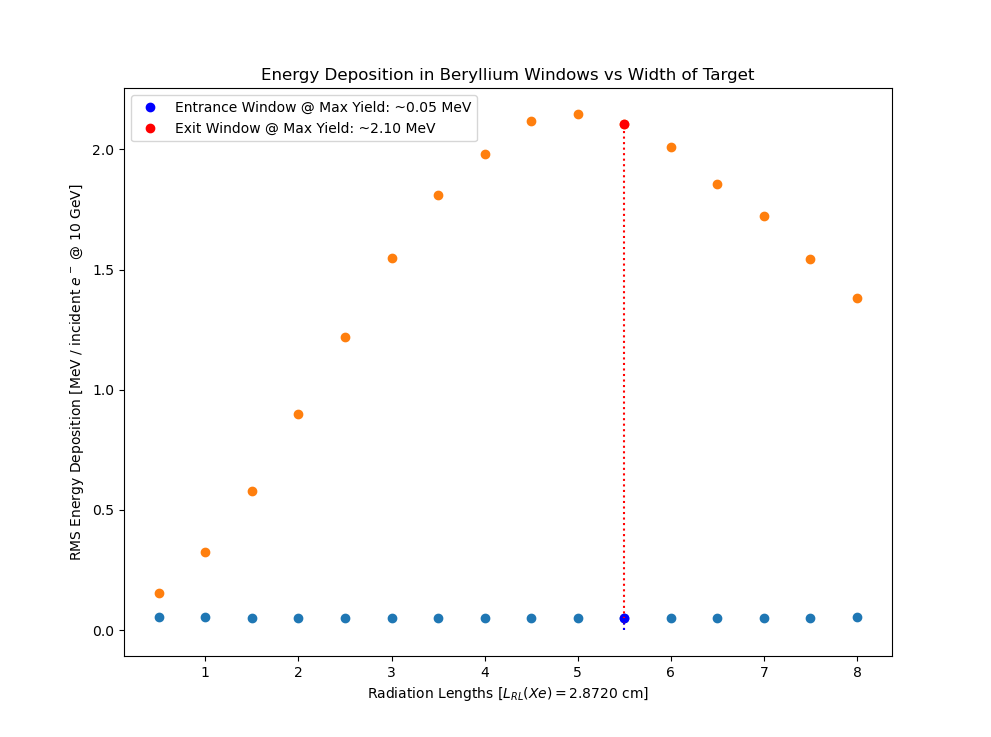
\includegraphics[width = .5\textwidth]{../images/WindowDeps.png}
    \caption{\label{fig:WinDeps}Energy deposition on incident and exit Beryllium windows.}
\end{figure}

\section{Conclusion}
\subsection{Design of Liquid Xenon Chamber}
Here we explore how one could design a chamber for the liquid Xenon target.

Source code and sample data for GEANT4 simulations can be found at 
\url{https://github.com/MaxVarverakis/LiquidXenonSims.git}.










\begin{acknowledgments}
We wish to acknowledge the support of the author community in using
REV\TeX{}, offering suggestions and encouragement, testing new versions,
\dots.
\end{acknowledgments}

\appendix
\section{Appendixes}

To start the appendixes, use the \verb+\appendix+ command.
This signals that all following section commands refer to appendixes
instead of regular sections. Therefore, the \verb+\appendix+ command
should be used only once---to setup the section commands to act as
appendixes. Thereafter normal section commands are used. The heading
for a section can be left empty. For example,
\begin{verbatim}
\appendix
\section{}
\end{verbatim}
will produce an appendix heading that says ``APPENDIX A'' and
\begin{verbatim}
\appendix
\section{Background}
\end{verbatim}
will produce an appendix heading that says ``APPENDIX A: BACKGROUND''
(note that the colon is set automatically).

If there is only one appendix, then the letter ``A'' should not
appear. This is suppressed by using the star version of the appendix
command (\verb+\appendix*+ in the place of \verb+\appendix+).

\section{A little more on appendixes}

Observe that this appendix was started by using
\begin{verbatim}
\section{A little more on appendixes}
\end{verbatim}

Note the equation number in an appendix:
\begin{equation}
E=mc^2.
\end{equation}

\subsection{\label{app:subsec}A subsection in an appendix}

You can use a subsection or subsubsection in an appendix. Note the
numbering: we are now in Appendix~\ref{app:subsec}.

Note the equation numbers in this appendix, produced with the
subequations environment:
\begin{subequations}
\begin{eqnarray}
E&=&mc, \label{appa}
\\
E&=&mc^2, \label{appb}
\\
E&\agt& mc^3. \label{appc}
\end{eqnarray}
\end{subequations}
They turn out to be Eqs.~(\ref{appa}), (\ref{appb}), and (\ref{appc}).

% The \nocite command causes all entries in a bibliography to be printed out
% whether or not they are actually referenced in the text. This is appropriate
% for the sample file to show the different styles of references, but authors
% most likely will not want to use it.
\nocite{*}

% \bibliography{apssamp}% Produces the bibliography via BibTeX.

\end{document}
%
% ****** End of file apssamp.tex ******
